\section{Der Elementarteilersatz}

Sei $R$ Hauptidealring.

\begin{definition}
	Seien $a,b,x,y\in R$. Für $i,j\in\{1,...,n\}$ ist
	\begin{align}
		E_{ij} = (\delta_{\sigma,i},...,\delta_{\mu,j})_{\sigma,\mu}\in\Mat_n(\real)\notag
	\end{align}
	Sei
	\begin{align}
		E_{ij}(a,b,x,y) = \mathbbm{1}_n-E_{ii}-E_{jj}+aE_{ii}+bE_{ij}+xE_{jj}+yE_{ji}\notag
	\end{align}
	%TODO: Matrix ergänzen von Pascal
\end{definition}

\begin{lemma}
	Ist $ax-by\in R^\times$, so ist
	\begin{align}
		E_{ij}(a,b,x,y)\in \GL_n(\real)\notag
	\end{align}
\end{lemma}
\begin{proof}
	Folgt aus LAAG1 IV.3.4, da
	%TODO: Verlinkung
	\begin{align}
		\det(E_{ij}(a,b,x,y))=ax-by\in R^\times\notag
	\end{align}
	Oder direkt: Das Inverse ist $E_{ij}(xc^{-1},bc^{-1}, ac^{-1},-yc^{-1})$, zum Beispiel
	\begin{align}
		\begin{pmatrix} a & b \\ y & x\end{pmatrix}\begin{pmatrix}xc^{-1} & -bc^{-1} \\ -yc^{-1} & ac^{-1}\end{pmatrix}=\begin{pmatrix}(ax-by)c^{-1} & 0 \\ 0 & (ax-by)c^{-1}\end{pmatrix}\notag
	\end{align}
\end{proof}

\begin{remark}
	Multiplikation von $E_{ij}(a,b,x,y)$ von links an $A$ führt eine Zeilenumformung durch: Sind $a_1,...,a_n$ die Zeilen von $A$, so wird $a_i$ durch $aa_i+ba_j$ ersetzt, und gleichzeitig $a_j$ durch $ya_i+xa_j$ ersetzt. Ist $ax-by=1$, so sind diese Zeilenumformungen invertierbar.
	
	\emph{Spezialfälle}: elementare Zeilenumformungen von Typ II und III aus Kapitel III (LAAG 1). Warnung: Im Gegensatz dazu sind über einem Ring $R$ die elementaren Zeilenumformungen vom Typ I (Multiplikation mit einem Skalar) nicht immer invertierbar!
	
	Multiplikation mit $E_{ij}(a,b,x,y)$ von rechts führt entsprechende Spaltenumformungen durch.
\end{remark}

\begin{theorem}[Elementarteilersatz für Matrizen, \person{Smith}-Normalform]
	\proplbl{8_6_4}
	Sei $A\in\Mat_{m\times n}(\real)$. Es gibt $0\le r \le\min\{n,m\}$, $S\in\GL_m(R)$, $T\in\GL_n(R)$
	mit 
	\begin{align}
		SAT &= \begin{pmatrix}d_1 & & & \\ & \ddots & & \\ & & d_r & \\ & & & \mathbb{0}\end{pmatrix} \notag \\
		\mathbb{0} &\in\Mat_{m-r\times n-r}\notag
	\end{align}
	wobei $d_i\in R\backslash\{0\}$ mit $d_i\mid d_{i+1}$ für $i=1,...,n-1$
\end{theorem}
\begin{proof}
	Induktion nach $\min\{m,n\}$. Für $a\in R$ sei $\delta(a)\in\natur_0\cup\{\infty\}$ die Anzahl der Primelemente in der Primfaktorzerlegung von $a$, mit $\delta(0):=\infty$, und $\delta(A):=\min_{ij}\{\delta(a_{ij})\}$. Wir können annehmen, dass $\delta(A)\le \delta(SAT)$ für alle $S\in \GL_m(R)$ und $T\in \GL_n(R)$. Durch Zeilen- und Spaltenvertauschungen erreichen wir, dass $\delta(a_{11})=\delta(A)$.
	\begin{itemize}
		\item \emph{1. Behauptung:} $a_{11}\mid a_{i1}$ für alle $i$. Gäbe es ein $i\ge 1$ für dass $a_{11}\nmid a_{i1}$, so sei $c=\ggT(a_{11},a_{i1})=xa_{11}+ya_{i1}$ mit $\ggT(x,y)=1$, also $ax-by=1$ mit $a,b\in R$. Multiplikation mit $E_{1i}(x,y,a,b)$ von links erzeugt an der Position $(1,1)$ das Element $c$, und $\delta(c)<\delta(a_{11})=\delta(A)$, im Widerspruch zur Minimalität von $\delta(A)$. \\
		Analog zeigt man, dass $a_{11}\mid a_{1j}$ für alle $j$. Durch Zeilen- und Spaltenumformungen können wir deshalb nun $a_{i1}=0$ für alle $i>1$ und $a_{1j}$ für alle $j>1$ erreichen.
		\item\emph{2. Behauptung:} $a_{11}\mid a_{ij}$ für alle $i,j$. Gäbe es $i>1$ und $j>1$ mit $a_{11}\nmid a_{ij}:=b$, so können wir die $j$-te Spalte zur ersten Spalte addieren, was $a_{11}$ nicht ändert und $a_{1i}=b$ bewirkt. Wider können wir Behauptung 1 anwenden und erhalten den Widerspruch, dass $a_{11}\mid b$. Damit ist nach diesem Umformungen
		\begin{align}
			A=\begin{pmatrix}a_{11} & \\ & a_{11}\cdot A'\end{pmatrix}\notag
		\end{align}
		mit $A'\in\Mat_{(m-1)\times (n-1)}(R)$. Wir wenden nun die Induktionshypothese auf $A'$ an und sind fertig.
	\end{itemize}
\end{proof}

\begin{mathematica}[\person{Smith}-Normalform]
	Elementarteiler einer Matrix $A$ lassen sich mit Mathematica mit der Funktion
	\begin{align}
	\texttt{SmithDecomposition[A]}\notag
	\end{align}
	die als einziges Argument eine Matrix braucht. Allerdings ist der Output unformatiert, mit folgenden Befehl sieht das deutlich besser aus:
	\begin{align}
	\text{\texttt{MatrixForm/@ (\{u,r,v\} = SmithDecomposition[A])}}\notag
	\end{align}
	Der Output sind 3 Matrizen, wobei \texttt{u} für $S$, \texttt{v} für $T$ und \texttt{r} für das Ergebnis von $SAT$ steht.
\end{mathematica}

\begin{remark}
	Man kann zeigen, dass die $d_1,...,d_r$ bis auf Assoziiertheit eindeutig bestimmt sind. Man nennt sie deshalb \begriff{Elementarteiler} der Matrix $A$.
\end{remark}

\begin{example}
	Sei $R=\whole$. Die Elementarteiler von
	\begin{align}
		A=\begin{pmatrix}2&0&0 \\ 0&4&0 \\0&0&6\end{pmatrix}\notag
	\end{align}
	sind 
	\begin{align}
		\begin{pmatrix}4&0\\0&6\end{pmatrix}\to\begin{pmatrix}4&0\\4&6\end{pmatrix}\notag
		\to\begin{pmatrix}4&0\\-2&6\end{pmatrix} \to\begin{pmatrix}2&-6\\4&0\end{pmatrix} \notag
		\to\begin{pmatrix}2&0\\4&12\end{pmatrix} \to\begin{pmatrix}2&0\\0&12\end{pmatrix}\notag
	\end{align}
	2, 2 und 12.
\end{example}

\begin{*anmerkung}[Teil 1]
	Um die Elementarteiler der Matrix $A_0$ zu ermitteln, muss man geschickt mit Matrizen $S$ und $T$ multiplizieren. Dazu starten wir links oben bei Element $a_{11}\neq 0$ und versuchen nun, auf der ersten Spalte und auf der ersten Zeile nur Nullen zu produzieren, aber $a_{11}\neq 0$ zu erhalten.
	
	 Dazu fangen wir mit der ersten Spalte an. Ziel ist es, das letzte Element dieser Spalte durch geschickte Addition der vorletzten Spalte zu 0 werden zu lassen. Wir schauen uns die letzten 2 Elemente, nennen wir sie $x$ und $y$, dieser ersten Spalte an und bestimmen $\ggT(x,y)$. Weiterhin suchen wir $u$ und  $v$, sodass folgende Gleichung erfüllt ist:
	\begin{align}
		\ggT(x,y)=u\cdot x + v\cdot y\notag
	\end{align}
	Da wir eine Zeilenoperation durchführen wollen, brauchen wir eine Matrix $S_0$, die wir von links an $A$ ranmultiplizieren. Dabei müssen wir auf die richtige Dimension von $S_0$ aufpassen. Dazu setzen wir $S_0$ auf $\mathbbm{1}_m$ und fügen an der richtigen Stelle die Matrix $S'_0$ ein:
	\begin{align}
		S'_0=\begin{pmatrix}u & v \\ -\frac{y}{\ggT(x,y)} & \frac{x}{\ggT(x,y)}\end{pmatrix}\notag
	\end{align}
	Jetzt bestimmen wir $A_1:=A_0\cdot S_0$. Jetzt haben wir das letzte Element der ersten Spalte zu 0 verwandelt. Wir arbeiten uns jetzt in der ersten Spalte nach oben, versuchen also das vorletzte Element zu 0 zu verwandeln, aber mithilfe der vorvorletzten Zeile. Auch dazu bestimmen wir wieder Matrizen $S_1,S_2,...$ bis die erste Spalte 0 ist, mit Ausnahme von $a_{11}$. 
\end{*anmerkung}
\begin{*anmerkung}[Teil 2]
	Jetzt wenden wir uns der ersten Zeile zu: Auch hier versuchen wir das letzte Element zu 0 zu verwandeln, aber eben mit Benutzung der vorletzten Spalte. Die Vorgehensweise ist nahezu identisch, wir bestimmen auch wieder $\ggT(x,y)$ und lösen
	\begin{align}
		\ggT(x,y)=u\cdot x + v\cdot y\notag
	\end{align}
	Damit bauen wir uns wieder $T'_0$, die wir an der passenden Stelle in $T_0=\mathbbm{1}_n$ einsetzen
	\begin{align}
		T'_0=\begin{pmatrix}u & -\frac{y}{\ggT(x,y)} \\ v & \frac{x}{\ggT(x,y)}\end{pmatrix}\notag
	\end{align}
	Die Matrix $T_0$ multiplizieren wir aber diesmal von rechts an $A_n$. So arbeiten wir uns wieder von hinten nach vorne. Es kann passieren, dass wir uns damit leider wieder in der ersten Spalte ein paar Nullen kaputt machen, aber dann bauen wir wieder eine $S_n$-Matrix mit der wieder Nullen erscheinen. Falls das wieder die Spalten kaputt macht, dann multiplizieren wir wieder mit einer $T_n$-Matrix. Das \propref{8_6_4} garantiert uns, dass wir irgendwann fertig werden.
\end{*anmerkung}
\begin{*anmerkung}[Teil 3]	
	Haben wir nun die erste Zeile und die erste Spalte zu 0 verwandelt, außer $a_{11}$ natürlich, kümmern wir uns um die Untermatrix in Richtung rechts unten. Hier geht der Algorithmus von vorne los; das Schöne ist, dass er uns die erste Zeile/Spalte nicht mehr kaputt machen kann. Irgendwann sind wir rechts unten angekommen und haben nur noch Elemente auf der Hauptdiagonalen stehen. Diese sollten, wie in \propref{8_6_4} behauptet eine solche Teilerkette bilden. Tun sie das nicht, kann man wieder mit Matrizen $S_n$ und $T_n$ nachhelfen.
	\begin{align}
		S'_n=\begin{pmatrix}u & v \\ -\frac{y}{\ggT(x,y)} & \frac{x}{\ggT(x,y)}\end{pmatrix}\quad 
		T'_n=\begin{pmatrix}1 & -\frac{vy}{\ggT(x,y)} \\ 1 & \frac{ux}{\ggT(x,y)}\end{pmatrix} \notag \\
		\text{unter Vorbehalt! }S'_n=\begin{pmatrix}1 & 1 \\ -\frac{vy}{\ggT(x,y)} & \frac{ux}{\ggT(x,y)}\end{pmatrix}\notag
	\end{align}
	Und dann sind wir endlich fertig! Die Transformationsmatrizen $S$ und $T$ sind dann einfach
	\begin{align}
		S = S_1\cdot S_2\cdot ... \notag \\
		T = T_1\cdot T_2\cdot ... \notag
	\end{align}
	Weitere Informationen und Beispiele findet man auf \url{http://www.igt.uni-stuttgart.de/eiserm/lehre/2010/Algebra/Matrizenringe.pdf}, ab Abschnitt §7D
\end{*anmerkung}

\begin{lemma}
	\proplbl{8_6_7}
	Ist $M$ ein endlich erzeugter freier $R$-Modul und $N\subseteq M$ ein Untermodul, so ist auch $N$ endlich erzeugt.
\end{lemma}
\begin{proof}
	Sei $(x_1,...,x_m)$ eine Basis von $M$. Induktion nach $m$. \\
	\emph{$m=1$:} Durch $1\mapsto x_1$ wird nach \propref{8_1_11} eine $R$-lineare Abbildung $f:R\to M$ gegeben, die ein Isomorphismus ist. Der Untermodul $N\subseteq M$ entspricht einem Ideal $I:=f^{-1}(N)$ von $R$. Da $R$ ein Hauptidealring ist, ist $I=(a)$ für ein $a\in R$, somit $N=f(I)=R\cdot f(a)$. Insbesondere ist $N$ endlich erzeugt, sogar von einem Element. \\
	\emph{$m-1\to m$:} Definiere $M'=\sum_{i=1}^{m-1}Rx_i$, $M''=Rx_m$, $N'=N\cap M'$. Sei unter $\pi: M\to M''$ die $R$-lineare Abbildung gegeben nach \propref{8_1_11} durch $\pi(x_i)=\delta_{i,m}x_m$. Nach Induktionshypothese ist $N'$ endlich erzeugt, etwa $N'=\sum_{j=1}^n Ry_j$. Aus dem Fall $m=1$ sehen wir zudem, dass $N''=\pi(N)=R\pi(y)$ für ein $y\in N$. Sei $\tilde{N}=Ry+\sum_{j=1}^n Ry_j\subseteq N$. Da $\Ker(\pi\vert_N)=M''\cap N=N'\subseteq\tilde{N}$ und $\pi\vert_N(\tilde{N})\supseteq R\pi(y)=N''=\pi\vert_N(N)$ ist $\tilde{N}=N$ nach \propref{8_5_5} und \propref{8_5_4}. Somit ist $N$ endlich erzeugt.
\end{proof}

\begin{proposition}[Elementarteilersatz für Moduln]
	\proplbl{8_6_8}
	Sei $R$ ein Hauptidealring, $M\cong R^m$ ein endlich erzeugter freier $R$-Modul, $N\subseteq M$ ein Untermodul. Dann existiert $r\in\natur$, eine Basis $B'=(x'_1,...,x'_m)$ von $M$ und $d_1,...,d_r\in R\backslash\{0\}$ mit $d_i\mid d_{i+1}$ für $i=1,...,r-1$ für die $(d_1x'_1,...,d_rx'_r)$ eine Basis von $N$ ist.
\end{proposition}
\begin{proof}
	Sei $B=(x_1,...,x_m)$ eine Basis von $M$. Nach \propref{8_6_7} ist $N$ endlich erzeugt, also 
	\begin{align}
		N=\sum_{j=1}^n Ry_j\quad\text{ mit }\quad y_j=\sum_{i=1}^m a_{ij}x_i\quad a_{ij}\in R\notag
	\end{align}
	Wir betrachten die lineare Abbildung $f:R^n\to M$ gegeben durch $f(e_j)=y_j$. Dann ist $\Image(f)=N$ und 
	\begin{align}
		M_B^{\mathcal{E}}(f)=A=(a_{ij})\in\Mat_{m\times n}(R)\notag
	\end{align}
	Nach \propref{8_6_4} existieren $S\in\GL_m(R)$, $T\in\GL_n(R)$ mit
	\begin{align}
		SAT=D=\diag(d_1,...,d_r,\mathbb{0})\notag
	\end{align}
	Es gibt somit Basen $\mathcal{E}'=(e'_1,...,e'_n)$ von $R^n$, $B'=(x'_1,...,x'_m)$ von $M$ mit $M_{B'}^{\mathcal{E}'}(f)=D$. Somit ist $N=\Image(f)=\sum_{i=1}^n R\cdot f(e'_i)=\sum_{j=1}^r Rd_jx'_j$. Da $(x'_1,...,x'_r)$ frei und $R$ nullteilerfrei ist, ist auch $(d_1x'_1,...,d_rx'_r)$ frei, also eine Basis von $N$.
\end{proof}

\begin{*example}
	Sei $R=\whole$, $M=\whole^2$, \textcolor{blue}{$N$ }$=\whole\begin{henrysmatrix}2\\0\end{henrysmatrix}+\whole\begin{henrysmatrix}1\\2\end{henrysmatrix}$
	\begin{align}
		&\begin{pmatrix}2&1\\0&2\end{pmatrix}\to\begin{pmatrix}1&2\\2&0\end{pmatrix}\to\begin{pmatrix}1&0\\2&-4\end{pmatrix}\to\begin{pmatrix}1&0\\0&4\end{pmatrix}\notag \\
		&\Rightarrow B = \left(\begin{henrysmatrix}1\\0\end{henrysmatrix},\begin{henrysmatrix}0\\4\end{henrysmatrix} \right)\Rightarrow \textcolor{red}{B'=\left(\begin{henrysmatrix}1\\2\end{henrysmatrix}, \begin{henrysmatrix}1\\1\end{henrysmatrix} \right)}\notag \\
		&\Rightarrow \textcolor{cyan}{C=\left(1\cdot\begin{henrysmatrix}1\\2\end{henrysmatrix},4\cdot \begin{henrysmatrix}1\\1\end{henrysmatrix} \right)}\text{ ist Basis von }\textcolor{blue}{N}\notag
	\end{align}
	\begin{center}
		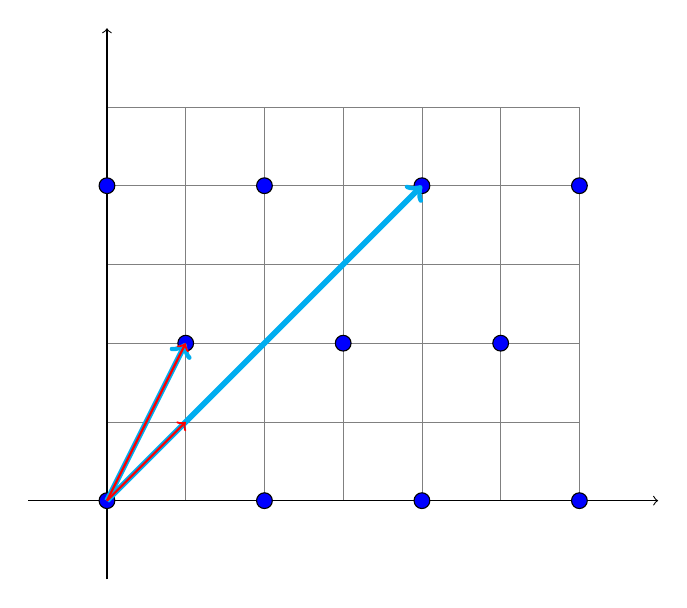
\begin{tikzpicture}
		\draw[help lines, line width=.2pt, step=1] (0,0) grid (6,5);
		\draw[->] (-1,0) -- (7,0);
		\draw[->] (0,-1) -- (0,6);
		\draw[fill=blue] (0,0) circle (0.1);
		\draw[fill=blue] (2,0) circle (0.1);
		\draw[fill=blue] (4,0) circle (0.1);
		\draw[fill=blue] (6,0) circle (0.1);
		\draw[fill=blue] (0,4) circle (0.1);
		\draw[fill=blue] (2,4) circle (0.1);
		\draw[fill=blue] (4,4) circle (0.1);
		\draw[fill=blue] (6,4) circle (0.1);
		\draw[fill=blue] (1,2) circle (0.1);
		\draw[fill=blue] (3,2) circle (0.1);
		\draw[fill=blue] (5,2) circle (0.1);
		\draw[->, cyan, line width=2pt] (0,0) -- (1,2);
		\draw[->, cyan, line width=2pt] (0,0) -- (4,4);
		\draw[->, red, thick] (0,0) -- (1,2);
		\draw[->, red, thick] (0,0) -- (1,1);
		\end{tikzpicture}
	\end{center}
\end{*example}

\begin{remark}
	Wieder kann man zeigen, dass $d_1,...,d_r$ bis auf Einheiten eindeutig bestimmt sind.
\end{remark}

\begin{conclusion}
	\proplbl{8_6_10}
	Ist $R$ ein Hauptidealring, so ist ein Untermodul eines endlich erzeugten freien $R$-Moduls wieder frei.
\end{conclusion}

\begin{remark}
	\propref{8_6_10} wird \emph{falsch} ohne "'$R$ Hauptidealring"'. So ist zum Beispiel $N=(x,y)\unlhd\ratio[x,y]=(\ratio[x])[y]=R=M$ kein Hauptideal und somit ein nicht freier Untermodul des freien $R$-Moduls $R$: Je zwei Elemente von $R$ sind linear abhängig, für $a,b\in R$ ist
	\begin{align}
		b\cdot a+(-a)\cdot b=0\notag
	\end{align}
	Deshalb kann $N$ keine Basis mit mehr als einem Element besitzen.
	
	Die Voraussetzung "'endlich erzeugt"' ist hingegen nicht notwendig, aber der Beweis wird dadurch einfacher. 
\end{remark}

\begin{conclusion}
	Ist $R$ ein Hauptidealring, so ist ein Untermodul eines endlich erzeugten $R$-Moduls $M$ wieder endlich erzeugt.
\end{conclusion}
\begin{proof}
	Ist $M=\sum_{j=1}^m Ry_j$, so betrachte die $R$-lineare Abbildung $f:R^m\to M$ gegeben durch $f(e_j)=y_j$ für $j=1,...,m$. Nach \propref{8_6_7} ist $f^{-1}(N)\subseteq R^m$ endlich erzeugt, etwa $f^{-1}(N)=\sum_{i=1}^n Rx_i$. Somit ist $N=f(f^{-1}(N))=\sum_{i=1}^n R\cdot f(x_i)$ endlich erzeugt.
\end{proof}

\begin{theorem}[Hauptsatz über endlich erzeugte Moduln über Hauptidealringen]
	\proplbl{8_6_13}
	Sei $R$ ein Hauptidealring und $M$ ein endlich erzeugter $R$-Modul. Dann ist
	\begin{align}
		M = F\oplus M_{tor}\notag
	\end{align}
	wobei $F\cong R^r$ ein endlich erzeugter freier $R$-Modul ist und
	\begin{align}
		M_{tor} \cong \bigoplus_{i=1}^n \qraum{R}{Rd_i}\notag
	\end{align}
	mit Nichteinheiten $d_1,...,d_n\in R\backslash\{0\}$, die $d_i\mid d_{i+1}$ für $i=1,...,n-1$ erfüllen.
\end{theorem}
\begin{proof}
	Sei $M=\sum_{j=1}^m Ry_j$. Betrachte die lineare Abbildung $f:R^m\to M$ gegeben durch $f(e_j)=y_j$ und dem Untermodul $N=\Ker(f)\subseteq R^m$. Nach \propref{8_6_8} existiert eine Basis $(x_1,...,x_s)$ von $R^m$, $n\le s$ und $d_1,...,d_n\in R\backslash\{0\}$ mit $d_i\mid d_{i+1}$ für die $(d_1x_1,...,d_nx_n)$ eine Basis von $N$ ist. Nach dem Homomorphiesatz ist
	\begin{align}
		M=\Image(f)&\cong\qraum{R^m}{N}=\qraum{\bigoplus_{i=1}^s Rx_i}{\bigoplus_{i=1}^n Rd_ix_i} \notag \\
		&\cong \qraum{R^s}{\bigoplus_{i=1}^n Rd_ie_i}\notag \\
		&\cong \bigoplus_{i=1}^n \qraum{R}{Rd_i}\oplus \underbrace{R^{s-n}}_{F}\notag
	\end{align}
	Ist $d_i\in R^\times$, so ist $\qraum{R}{Rd_i}=0$, wir können diese $i$ daher weglassen. Dabei ist $\bigoplus_{i=1}^n \qraum{R}{Rd_i}$ genau der Torsionsmodul $M_{tor}$:
	\begin{itemize}
		\item "'$\subseteq$"': Mit $d:=d_1\cdot ... \cdot d_n\in R\backslash\{0\}$ ist $d\cdot (x_i)_{1,...,n}=(dx_i)_{1,...,n}=(0,...,0)$ (Vielfache von $Rd_i$ machen das Element zu 0)
		\item "'$\supseteq$"': Ist $d\in R\backslash\{0\}$, $x\in\bigoplus_{i=1}^n\qraum{R}{Rd_i}$, $y\in R^{s-n}$ mit $d\cdot (x,y)=0$, so ist $d\cdot y=0$ und deshalb $y=0$.
	\end{itemize}
\end{proof}

\begin{remark}
	Auch hier sind $d_1,...,d_n$ (bis auf Einheiten) sowie $r$ eindeutig bestimmt. Man nennt $r$ den \begriff[Modul!]{(freien) Rang} von $M$.
\end{remark}

\begin{example}
	Eine endlich erzeugte abelsche Gruppe $A$ ist von der Form
	\begin{align}
		A\cong \whole^r\oplus\bigoplus_{i=1}^k \qraum{\whole}{d_i\whole}\notag
	\end{align}
	mit (eindeutig bestimmten) $d_1,...,d_k\in\natur$, $d_1\mid d_2\mid ...\mid d_k$.
\end{example}